\section{CP Modeling}

The first part technique used to approach the problem was to model it with CP (Constraint Programming) using Minizinc. CP is a declarative programming paradigm where the solver tries to find a solution (if this exists) by assigning a value to each variable, in a way that all the defined constraints are satisfied.

Before proceeding with the model definition it is worth noting that the instances were provided in text files, hence it was necessary to first convert them into .dzn data files, which are readable by Minizinc.

\subsection{Parameters and variables}

First of all, all the parameters, decision variables and objective variables of the problem had to be defined. 

In particular, we are given the following .dzn input data file:

$w = {width} \\
n = {number \; of \; circuits} \\
x\_sizes = [{x_0}, \; {x_1}, \; ..., \; {x_n}] \\
y\_sizes = [{y_0}, \; {y_1}, \; ..., \; {y_n}]$ \\

where:
\begin{itemize}
    \item $w$ is the plate width
    \item $n$ is the number of circuits to place in the plate
    \item $x\_sizes$ and $y\_sizes$ are two arrays with the horizontal and vertical sizes of the circuits, respectively (indexed from 1 to the number of circuits)
\end{itemize}\

Therefore, the same \textbf{input parameters} have been defined in the model using the Minizinc syntax:

\begin{verbatim}
int: width;
int: n;
set of int: CIRCUITS = 1..n; 

array[CIRCUITS] of int: x_sizes; 
array[CIRCUITS] of int: y_sizes; 
\end{verbatim}


\\

As for the \textbf{output parameters}, two parameters x and y were defined, indexed from 1 to n: each element i of the arrays contains the horizontal and vertical coordinates of the bottom-left corner of the i-th circuit, respectively:

\begin{verbatim}
array[CIRCUITS] of var 0..width-1: x
array[CIRCUITS] of var 0..sum(y_sizes)-1: y;
\end{verbatim}

\subsection{Domain reduction}

The \textbf{domain reduction contraints} allow to make the model more efficient by reducing the variable domain. This is done by defining a range for each variable of the array x: the bottom left corner of each rectangle i cannot be placed farther along the x axis than the plate width minus its width, otherwise it would fall outside the plate. A similar constraint can be defined for the domain of the y variables: the bottom left corner of each rectangle i cannot be placed higher on the y axis than the height of the plate minus its height.

\begin{verbatim}
constraint forall(i in CIRCUITS) (x[i] <= width - x_sizes[i])::domain; 
constraint forall(i in CIRCUITS) (y[i] <= height - y_sizes[i])::domain;
\end{verbatim}

Moreover, with the same purpose of reducing variables domain, upper and lower bounds were defined for the plate's height:
\begin{itemize}
    \item lower bound: the plate's height must be bigger than the height of the tallest rectangle
    \[ int: \; lowb = max(y\_sizes); \]
    \item upper bound: the plate's height must be below the sum of all the heights of each rectangle
    \[int: \; upb = sum(y\_sizes); \]
\end{itemize}


The \textbf {objective variable} is \textit{height}, which is the height of the plate: it is the variable to be minimised by the model during search. It ranges from the lower to the upper bound and is defined as:

\begin{verbatim}
var lowb..upb: height;
height = max([y[i] + y_sizes[i] | i in CIRCUITS]);
\end{verbatim}

\subsection{Constraints}

One of the most important parts of the problem is related to the definition of multiple constraints and their propagation in order to remove inconsistent values from variables domain.
The use of \textbf{global constraints} is useful for the solution of this problem, since it allows to obtain more efficient solutions thanks to propagation algorithms. Two different global constraints were used: \textbf {cumulative} and \textbf {diffn}. 

The cumulative constraint was taken from the modeling of scheduling problem: indeed it is usually used when we want you need to constraint the usage of shared resources by different tasks. In general, it requires that a set of tasks given by start times \textbf{s}, durations \textbf{d}  and resource requirements \textbf{r} never require more than a global resource bound \textbf{b} at any one time. 
Our problem can be seen as the one where there is a fixed capacity resource (plate width/height) and each task (circuit) has its own start time (placement) and duration (width/height). The constraint is repeated twice, once along each axis.

\begin{verbatim}
constraint cumulative(y, y_sizes, x_sizes, width); 
constraint cumulative(x, x_sizes, y_sizes, height);
\end{verbatim}

The diffn constraint is is a non-overlapping constraint which holds if, for each pair of shapes, there exists a dimension in which their projections don't overlap. Given the vectors of x and y bottom-left coordinates and the vectors of x and y sizes, with the diffn constraint we prevent the circuits from overlapping.

\begin{verbatim}
constraint diffn(x, y, x_sizes, y_sizes); 
\end{verbatim}


Furthermore, \textbf{symmetry braking constraints} were applied to reduce the number of solutions: the solver may in fact explore many symmetric variants of the same solution. The basic idea behind symmetry breaking is to impose an order.
In our case it was decided to place always the biggest circuit in the bottom left part
of the plate. To do this we need to define an order of the circuits, which is done by sorting them in descending order considering their area, given by the product between $x\_sizes$ and $y\_sizes$.

\begin{verbatim}
array [CIRCUITS] of  int: ord_circ = sort_by(CIRCUITS, area);
\end{verbatim}

After that we use the global constraint \textit{lex\_lesseq} on the coordinates of the circuits: This requires that the array x is lexicographically less than or equal to array y. It compares them from first to last element, regardless of indices.

\begin{verbatim}
constraint symmetry_breaking_constraint(
    let {
        int: c1 = ord_circ[1], int: c2 = ord_circ[2]
    } in lex_lesseq([y[c1],x[c1]], [y[c2],x[c2]])
);
\end{verbatim}

\subsection{Search}

Different combinations of search heuristics, for variables and domains, as well as restart strategies were employed to compare the model performances: \textit{input\_order}, \textit{first\_fail} and \textit{dom\_w\_deg} for variables (which specify the order in which the values should appear in the search tree), and \textit{indomain\_min} for domain (which specify which choice of value for each variable will be explored next).

More specifically, \textit{dom\_w\_deg} will choose the variable with the smallest value of domain size divided by weighted degree, which is the number of times it has been in a
constraint that caused failure earlier in the search. \textit{indomain\_min} will assign the variable its smallest domain value.

Also, restarting the search is useful to introduce randomness and break deterministic behaviour in searching solutions. In the model, different restart strategies were chosen:
\begin{itemize}
    \item restart\_constant(100)
    \item restart\_linear(100)
    \item restart\_geometric(1.5, 100)
    \item restart\_luby(100)
\end{itemize}

\subsection{Rotation model}

In the case we decided to take rotation of the circuits into account we should perform some modifications to the model. This is done by introducing a boolean array indexed by the number of circuits which specifies if each circuit is rotated or not:

\begin{verbatim} 
array[CIRCUITS] of var bool: rotation;
\end{verbatim} 

In case of rotation each rectangle will have its height and width swapped, therefore we need to update their actual values of widths and heights accordingly:

\begin{equation*}
\forall i \; in \; 1..n \; \; x\_sizes\_rot  = \begin{cases} y\_sizes[i] & \mbox{if } \mbox{rotation[i]} \\ x\_sizes[i] & \mbox{otherwise}\end{cases}
\end{equation*}

\begin{equation*}
\forall i \; in \; 1..n \; \; y\_sizes\_rot  = \begin{cases} x\_sizes[i] & \mbox{if } \mbox{rotation[i]} \\ y\_sizes[i] & \mbox{otherwise}\end{cases}
\end{equation*}

The objective function \textit{height} and the constraints seen before are modified with the vectors $x_sizes_rot$ and $y_sizes_rot$ to take rotation into account. We also introduce a new constraint: a circuit cannot be rotated if its height is greater than the plate width.

\begin{verbatim}
    constraint forall(i in CIRCUITS)(y_sizes[i] > width -> rotation[i]==false);
\end{verbatim}

The output file is also modified so that the string \textit{"rotated"} is printed next to the coordinates of the output circuits: this indicates that the relative circuit has been rotated. 

As an example, a possible output for the instance 3 is the following:

$ 10 \quad 10 \\
6 \\
3 \quad 3 \quad 3 \quad 4 \\
3 \quad 4 \quad 6 \quad 4 \quad rotated \\
3 \quad 6 \quad 0 \quad 4 \\
3 \quad 7 \quad 3 \quad 7 \quad rotated \\
4 \quad 4 \quad 0 \quad 0 \\
4 \quad 6 \quad 4 \quad 0 \quad rotated $ 

\newpage

\subsection{Results}

\begin{center}
\begin{longtable}{|l|l|l|}
\caption{Solving times obtained by CP models (without and with rotation)} \label{tab:long} \\

\hline \multicolumn{1}{|c|}{\textbf{Instance}} & \multicolumn{1}{c|}{\textbf{No rotation}} & \multicolumn{1}{c|}{\textbf{Rotation}} \\ \hline 
\endfirsthead

\multicolumn{3}{c}%
{{\bfseries \tablename\ \thetable{} -- continued from previous page}} \\
\hline \multicolumn{1}{|c|}{\textbf{Instance}} & \multicolumn{1}{c|}{\textbf{No rotation}} & \multicolumn{1}{c|}{\textbf{Rotation}} \\ \hline 
\endhead

\hline \multicolumn{3}{|r|}{{Continued on next page}} \\ \hline
\endfoot

\hline \hline
\endlastfoot

1 & 0,221 & 0,206 \\
2 & 0,202 & 0,206 \\
3 & 0,204 & 0,207 \\
4 & 0,203 & 0,275 \\
5 & 0,202 & 1,807 \\
6 & 0,200 & 0,561 \\
7 & 0,203 & 45,16 \\
8 & 0,201 & 0,246 \\
9 & 0,200 & 7,909 \\
10 & 0,205 & - \\
11 & 0,198 & - \\
12 & 0,208 & 0,234 \\
13 & 0,200 & - \\
14 & 0,237 & - \\
15 & 0,249 & 0,254 \\
16 & - & - \\
17 & 6,086 & 0,273 \\
18 & 1,422 & 1,234 \\
19 & - & - \\
20 & 5,687 & - \\
21 & 0,204 & - \\
22 & - & - \\
23 & 0,225 & - \\
24 & 0,209 & 0,279 \\
25 & - & - \\
26 & 147,1 & 1,755 \\
27 & 0,219 & 0,205 \\
28 & 16,68 & - \\
29 & 0,222 & - \\
30 & - & - \\
31 & - & - \\
32 & - & - \\
33 & 0,221 & 0,229 \\
34 & - & - \\
35 & - & - \\
36 & 0,259 & - \\
37 & - & - \\
38 & - & - \\
39 & - & - \\
40 & - & - \\
\end{longtable}
\end{center}

As shown in the table, the model without rotation is able to solve more instances within the time limit of 300 seconds, compared to the rotation model. Moreover, after performing different experiments with search heuristics and restart strategies, the best configuration turned out to be $input\_order$ and $indomain\_min$ with $restart\_geometric(1.5,500)$.

\newpage

\begin{figure}[!tbp]
  \centering
  \subfloat[Solution without rotation]{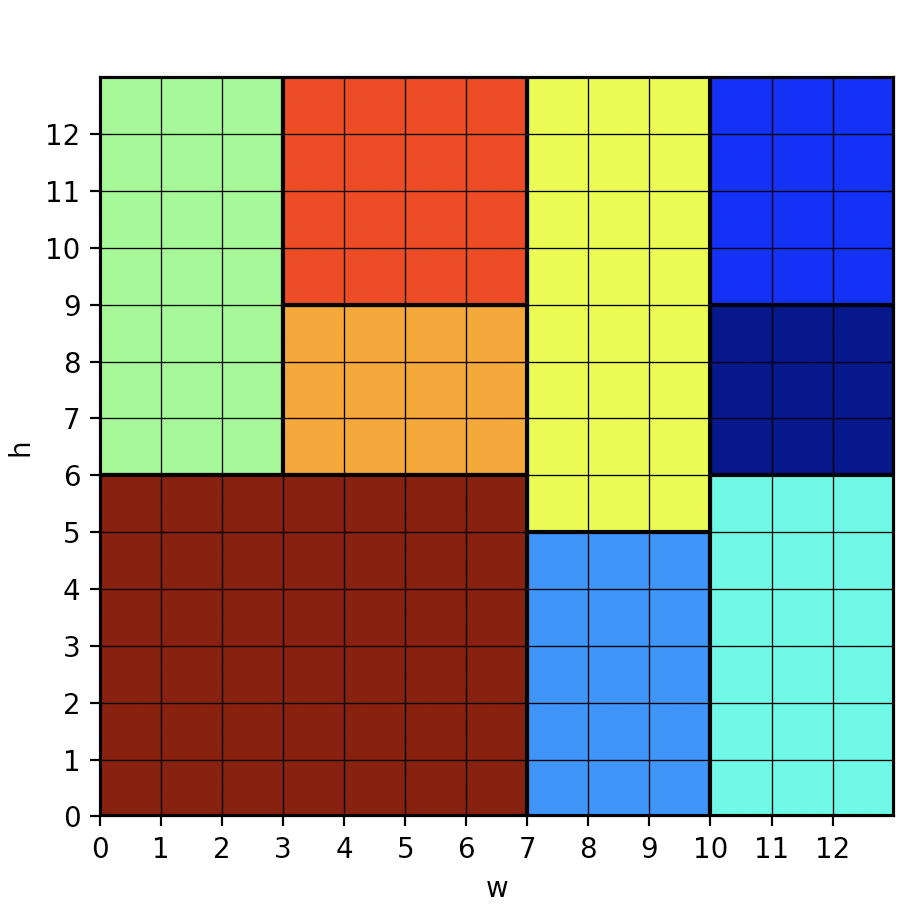
\includegraphics[width=0.4\textwidth]{Images/ins6.png}\label{fig:f1}}
  \hfill
  \subfloat[Solution with rotation]{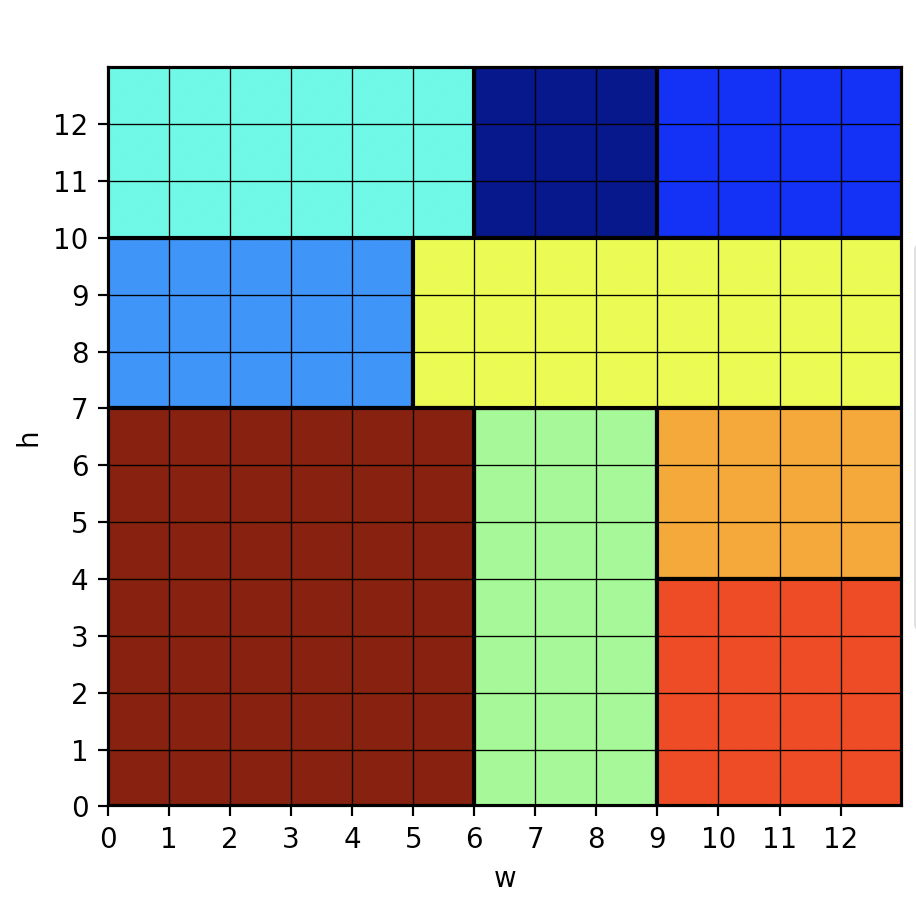
\includegraphics[width=0.4\textwidth]{Images/ins6-rot.png}\label{fig:f2}}
  \hfill
  \subfloat[Legend of circuits]{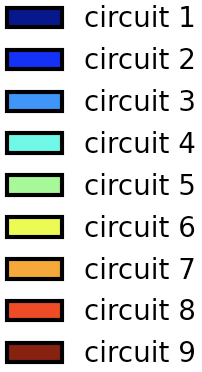
\includegraphics[width=0.1\textwidth]{Images/legend-ins6.png}\label{fig:f3}}
  \caption{Example of a possible solution for the instance n. 6}
\end{figure}